
\vspace{-5mm}
Amidakuji is a custom in Japan which 
allows for a pseudo-random assignment of children to prizes~\cite{A1}. 
Usually done in Japanese schools, a teacher will draw $n$ vertical lines, 
hereby known as \emph{lines}, where $n$ is the number of students in class. 
At the bottom of each line will be a unique prize. At the top of each line will be the name of one of the students.  
The teacher will then draw 0 or more horizontal lines, hereby known as \emph{bars}, 
connecting two adjacent lines. No two endpoints of two bars can be touching. 
The more bars there are the more complicated (and fun) 
the Amidakuji is. Each student then traces 
their line, and whenever they encounter an end point of a bar along their line, 
they must cross the bar and continue going down the adjacent line. 
The student continues tracing down the lines and crossing bars 
until they get to the end of the ladder lottery. We call such a tracing for a given student 
a \emph{path}. For example, the path of Ryu in the ladder lottery depicted in Figure~\ref{fig:aa} is highlighted in red. 
%%The prize at the bottom of the ladder lottery, at the end of a student's path, is their prize. 
\begin{center}
\vspace{-5mm}
\begin{figure}[h]
	\centering
		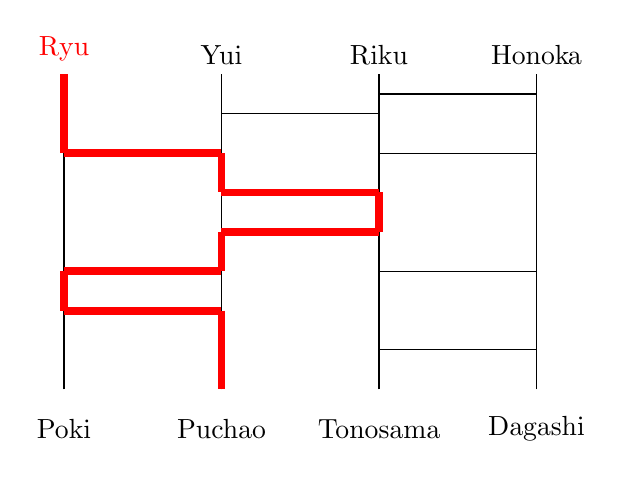
\begin{tikzpicture}
		%%Start of figure. Fig 1
			\draw(0, 0) to (0, 3); 
		
			\node at (0, -0.5){Poki};
			\draw(2, 0) to (2, 4) node[above]{Yui};
			\node at (2, -0.5){Puchao};
			\draw(4, 0) to (4, 4)node[above]{Riku};
			\node at (4, -0.5){Tonosama};
			\draw(6, 0) to (6, 4)node[above]{Honoka};
			\node at (6, -0.5){Dagashi};
			
			%bars%
		    \draw[line width=1mm, red](0, 3) to (0, 4) node[above]{Ryu};
			\draw[line width=1mm, red](0, 1) to (2, 1);
			\draw[line width=1mm, red](2, 1.5) to (2, 2);
			\draw[line width=1mm, red](0, 1)to(0, 1.5);
			\draw[line width=1mm, red](2, 1) to (2, 0);
			\draw[line width=1mm, red](0, 3) to (2, 3);
			\draw[line width=1mm, red](2, 3) to (2, 2.5);
			\draw[line width=1mm, red](4, 2) to (4, 2.5);
			\draw[line width=1mm, red](0, 1.5) to (2, 1.5);
			
			\draw[line width=1mm, red](2, 2) to (4, 2);
			\draw[line width=1mm, red](2, 2.5) to (4, 2.5);
			\draw(2, 3.5) to (4, 3.5);
			
			\draw(4, 0.5) to (6, 0.5);
			\draw(4, 3) to (6, 3);
			\draw(4, 1.5) to (6, 1.5);
			\draw(4, 3.75) to (6, 3.75);
		\end{tikzpicture}
\caption{A ladder lottery where Ryu gets Puchao, Yui gets Dagashi, Riku gets Tonosama and Honoka gets Poki}
\label{fig:aa}
\end{figure}
\end{center}
The term ``Amidakuji" has an interesting history. Amida is the Japanese name 
for Amithaba, the supreme Buddha of the Western Paradise. Amithaba
was a Buddha from India and there was a cult based around him. The cult 
of Amida, otherwise known as Amidism, believed that by worshiping Amithaba, they would 
enter into his Western paradise~\cite{A0}. Amidism began in India in the fourth century,
made its way to China and Korea in the fifth century, and finally came 
to Japan in ninth century. Kuji is the Japanese word for lottery. Hence, the game 
was termed Amidakuji. In English, Amidakuji translates to ladder lottery.\par 
The game Amidakuji began in Japan during 
the Muromachi period, which spanned from
1336 to 1573. During the Muromachi period, the game was played by having
players draw their names at the top of the lines, and at the bottom 
of the lines were pieces of paper that had the amount the players
were willing to bet. The pieces of paper were folded in the shape of 
Amithaba's halo~\cite{A0}. In Figure~\ref{Fig:Amida} a picture of Buddha Amithaba is provided.
\begin{figure}[ht]
	\centering 
	\resizebox{.3\textwidth}{.3\textheight}{
		\includegraphics{220px-Buddha_Amithaba.jpg}
	}
	\caption{Buddha Amida}
	\label{Fig:Amida}
\end{figure}

An interesting property about a ladder lottery is that it is  
associated with a \emph{permutation}. A \emph{permutation} is a unique ordering of objects. 
For the purposes of this thesis, the objects of a permutation are $1,2, \dots ,n$. 
A ladder lottery corresponds to a unique permutation $\pi$ when:
\begin{enumerate}
	\item The $n$ elements of $\pi$ are listed at the top of the ladder lottery in the order that they appear in 
	$\pi$; one element per line of the ladder lottery.
	\item At the bottom of the ladder lottery are the $n$ elements of $\pi$ in strictly ascending order. For 
	each element $x$ in $\pi$, $x$ goes down its path and ends up in the bottom $xth$ line.
	\item Each bar in the ladder is given a \emph{label} defined by two unique elements in $\pi$, $x>y$, which interchange at that specific bar. We draw 
	the label as $(x,y)$. 
\end{enumerate} 

% \begin{figure}[h]
% 	\centering
% 	\begin{tikzpicture}
% 		\draw(0, 0) to (0, 4);
% 			\draw(0, 3) to (1, 3);
% 		\draw(1, 0) to (1, 4);
% 			\draw(1, 2) to (2, 2);
% 		\draw(2, 0) to (2, 4);
% 			\draw(2, 3) to (3, 3);
% 		\draw(3, 0) to (3, 4);
		
% 		\draw(5, 0) to (5, 4);
% 			\draw(5, 3) to (6, 3);
% 		\draw(6, 0) to (6, 4);
% 			\draw[dashed](5, 2)--(8, 2);
% 			\draw(6, 1.5) to (7, 1.5);
% 		\draw(7, 0) to (7, 4);
% 			\draw(7, 3) to (8, 3);
% 		\draw(8, 0) to (8, 4);


% 		\draw(10, 0) to (10, 4);
% 			\draw(10, 3) to (11, 3);
% 		\draw(11, 0) to (11, 4);
% 			\draw(11, 2) to (12, 2);
% 		\draw(12, 0) to (12, 4);
% 			\draw(12, 3.5) to (13, 3.5);
% 		\draw(13, 0) to (13, 4);


% 		\node at(0, 4.3){\small{$3$}};
% 		\node at(1, 4.3){\small{$1$}};
% 		\node at(2, 4.3){\small{$4$}};
% 		\node at(3, 4.3){\small{$2$}};
		
% 		\node at(5, 4.3){\small{$3$}};
% 		\node at(6, 4.3){\small{$1$}};
% 		\node at(7, 4.3){\small{$4$}};
% 		\node at(8, 4.3){\small{$2$}};
		
% 		\node at(10, 4.3){\small{$3$}};
% 		\node at(11, 4.3){\small{$1$}};
% 		\node at(12, 4.3){\small{$4$}};
% 		\node at(13, 4.3){\small{$2$}};

% 		\node at(0, -.3){\small{$1$}};
% 		\node at(1, -.3){\small{$2$}};
% 		\node at(2, -.3){\small{$3$}};
% 		\node at(3, -.3){\small{$4$}};
		
% 		\node at(5, -.3){\small{$1$}};
% 		\node at(6, -.3){\small{$2$}};
% 		\node at(7, -.3){\small{$3$}};
% 		\node at(8, -.3){\small{$4$}};
		
% 		\node at(10, -.3){\small{$1$}};
% 		\node at(11, -.3){\small{$2$}};
% 		\node at(12, -.3){\small{$3$}};
% 		\node at(13, -.3){\small{$4$}};

% 		\node at(-1, 3){\small{Row $1$}};
% 		\node at(-1, 2){\small{Row $2$}};


% 		\node at(4, 3){\small{Row $1$}};
% 		\node at(4, 2){\small{Ghost Row $1$}};
% 		\node at(4, 1.5){\small{Row $2$}};


% 		\node at(9, 3.5){\small{Row $1$}};
% 		\node at(9, 3){\small{Row $2$}};
% 		\node at(9, 2){\small{Row $3$}};
% 	\end{tikzpicture}
% 	\caption{Three equivalent ladders. Leftmost and middle ladders are identical.}
% 	\label{Fig:equivLadders}
% \end{figure}


\section{Optimal Ladder Lotteries}
Consider a permutation $\pi=(p_{1},p_{2}, \dots ,p_{n})$.
A pair of elements, $p_{i}$ and $p_{j}$, form an \emph{inversion} if $p_{i}>p_{j}$ and $i<j$. 
For example, given $\pi=(4,3,5,1,2)$, its inversions are $(4,3),(4,2),(4,1),(3,2),(3,1),(5,1),(5,2)$.
A \emph{transposition} is a swap of two elements in $\pi$.
An \emph{adjacent transposition} is defined as a swap of two adjacent elements in $\pi$.
Given $\pi_{1}=(4,3,5,1,2)$ and $\pi_{2}=(3,4,5,1,2)$, they differ by the adjacent 
transposition of the elements $(4,3)$.
Let $k$ denote the number of inversions for some permutation.
An \emph{optimal ladder lottery} is a special case of ladder 
lottery, in which the number of bars equals the number of inversions in $\pi$. 
An optimal ladder lottery sorts $\pi$ in ascending order using exactly $k$ bars by applying 
$k$ adjacent transpositions on $k$ inversions in $\pi$. When a permutation has $k$ inversions, each bar 
transposes a single inversion in $\pi$ exactly once~\cite{A1}.
For example, given $\pi=(4,3,5,1,2)$ an optimal ladder lottery associated with $\pi$ would have 
seven bars; one for each inversion in $\pi$. For each bar, two elements in $\pi$ that form 
an inversion cross the given bar. 
Once all elements have crossed their respective bars, $\pi$ is sorted in ascending order. The number of bars in an optimal ladder lottery 
is the minimum number of bars in a ladder lottery required to sort $\pi$. 
To see an example of two ladder lotteries associated with 
$\pi=(4,3,5,1,2)$, one optimal and one non-optimal, please refer to Figure~\ref{fig:ab}.\par
\begin{figure}[h]
	\begin{minipage}{0.4\textwidth}
		\centering
		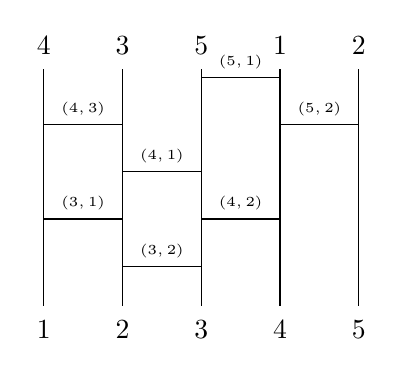
\begin{tikzpicture}
		 	\draw(0, 0) to (0, 3);
		 		\draw(0, 2.3) to (1, 2.3);
		 		\draw(0, 1.1) to (1, 1.1);

		 	\draw(1, 0) to (1, 3);
				 \draw(1, 1.7) to (2, 1.7);
				 \draw(1, .5) to (2, .5);
		 	\draw(2, 0) to (2, 3);
				 \draw(2, 2.9) to (3, 2.9);
				 \draw(2, 1.1) to (3, 1.1);
			 \draw(3, 0) to (3, 3);
			 	\draw(3, 2.3) to (4, 2.3);
			 \draw(4,0) to (4, 3);

			 \node at(0, 3.3){$4$};
			 \node at(1, 3.3){$3$};
			 \node at(2, 3.3){$5$};
			 \node at(3, 3.3){$1$};
			 \node at(4, 3.3){$2$};
			 \node at(0, -.3){$1$};
			 \node at(1, -.3){$2$};
			 \node at(2, -.3){$3$};
			 \node at(3, -.3){$4$};
			 \node at(4, -.3){$5$};

			 \node at(.5, 2.5){\tiny{$(4,3)$}};
			 \node at(.5, 1.3){\tiny{$(3,1)$}};
			 \node at(1.5, 1.9){\tiny{$(4,1)$}};
			 \node at(1.5, .7){\tiny{$(3,2)$}};
			 \node at(2.5, 3.1){\tiny{$(5,1)$}};
			 \node at(2.5, 1.3){\tiny{$(4,2)$}};
			 \node at(3.5, 2.5){\tiny{$(5,2)$}};


		\end{tikzpicture}
				

	\end{minipage}
	\begin{minipage}{.4\textwidth}
		\begin{flushright}
		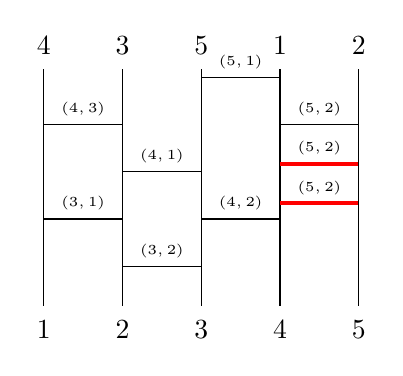
\begin{tikzpicture}
		 	\draw(0, 0) to (0, 3);
		 		\draw(0, 2.3) to (1, 2.3);
		 		\draw(0, 1.1) to (1, 1.1);

		 	\draw(1, 0) to (1, 3);
				 \draw(1, 1.7) to (2, 1.7);
				 \draw(1, .5) to (2, .5);
		 	\draw(2, 0) to (2, 3);
				 \draw(2, 2.9) to (3, 2.9);
				 \draw(2, 1.1) to (3, 1.1);
			 \draw(3, 0) to (3, 3);
				 \draw(3, 2.3) to (4, 2.3);
				 \draw [line width=0.5mm, red ](3, 1.8) to (4, 1.8);
				 \draw[line width=0.5mm, red ](3, 1.3) to (4, 1.3);
			 \draw(4,0) to (4, 3);

			 \node at(0, 3.3){$4$};
			 \node at(1, 3.3){$3$};
			 \node at(2, 3.3){$5$};
			 \node at(3, 3.3){$1$};
			 \node at(4, 3.3){$2$};
			 \node at(0, -.3){$1$};
			 \node at(1, -.3){$2$};
			 \node at(2, -.3){$3$};
			 \node at(3, -.3){$4$};
			 \node at(4, -.3){$5$};


			 \node at(.5, 2.5){\tiny{$(4,3)$}};
			 \node at(.5, 1.3){\tiny{$(3,1)$}};
			 \node at(1.5, 1.9){\tiny{$(4,1)$}};
			 \node at(1.5, .7){\tiny{$(3,2)$}};
			 \node at(2.5, 3.1){\tiny{$(5,1)$}};
			 \node at(2.5, 1.3){\tiny{$(4,2)$}};
			 \node at(3.5, 2.5){\tiny{$(5,2)$}};
			 \node at(3.5, 2.0){\tiny{$(5,2)$}};
			 \node at(3.5, 1.5){\tiny{$(5,2)$}};



		\end{tikzpicture}
	\end{flushright}
	\end{minipage}
	\caption{Two ladders for the permutation $(4,3,5,1,2)$. The left ladder is an optimal ladder and the right ladder is not. 
	The bold  bars in the right ladder are redundant, thus the right ladder is non optimal.}
	\label{fig:ab}
\end{figure}
Let $OptL\{\pi\}$ be defined as the set of optimal ladder lotteries for a specific $\pi$. The first discussion of 
$OptL\{\pi\}$ is in the paper Efficient Enumeration of Ladder Lotteries and its Application~\cite{A1}.
In this paper, the authors provide an algorithm 
which generates $OptL\{\pi\}$; the details of the algorithm are discussed in Chapter 2.
To see $OptL\{(4,3,5,1,2)\}$ please refer to Figure \ref{Fig:OptL3421}.
Given that there are $n!$ permutations of order $n$, each of them 
have their own $OptL\{\pi\}$. In Table~\ref{table:KInvOptL} found in the section A.1 of the Appendix 
the number of ladders in each $OptL\{\pi\}$ of order $5$ is presented. In general, 
$|OptL\{(n,n-1, \dots, 2,1)\}|$ is maximal with respect to a permutation of order $n$. When $n=5$, $|OptL\{(5,4,3,2,1)\}|=62$.
\begin{figure}[h]
	\centering
	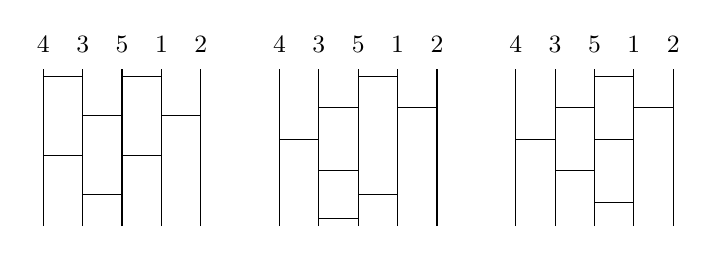
\begin{tikzpicture}
		\draw(0,0) to (0,2);
			\draw(0, 1.9) to (.5, 1.9);
			\draw(0, .9) to (.5, .9);
		\draw(.5,0) to (0.5,2);
			\draw(.5, 1.4) to (1, 1.4);
			\draw(.5, .4) to (1, .4);
		\draw(1,0) to (1,2);
			\draw(1, 1.9) to (1.5, 1.9);
			\draw(1, .9) to (1.5, .9);
		\draw(1.5,0) to (1.5,2);
			\draw(1.5, 1.4) to (2, 1.4);
		\draw(2,0) to (2,2);

		\draw(3, 0) to (3, 2);
			\draw(4, 1.9) to (4.5, 1.9);
			\draw(3.5, 1.5) to (4, 1.5);
			\draw(4.5, 1.5) to (5, 1.5);
			\draw(3.5, 1.1) to (3, 1.1);
			\draw(3.5, 0.7) to (4, 0.7);
			\draw(4, .4) to (4.5, .4);
			\draw(3.5, .1) to (4, .1);
		\draw(3.5, 0) to (3.5, 2);
		\draw(4, 0) to (4, 2);
		\draw(4.5, 0) to (4.5, 2);
		\draw(5, 0) to (5, 2);

		\draw(6, 0) to (6, 2);
			\draw(7.5, 1.9) to (7, 1.9);
			\draw(6.5, 1.5) to (7, 1.5);
			\draw(7.5, 1.5) to (8, 1.5);
			\draw(6, 1.1) to (6.5, 1.1);
			\draw(7, 1.1) to (7.5, 1.1);
			\draw(6.5, 0.7) to (7, 0.7);
			\draw(7, 0.3) to (7.5, 0.3);
		\draw(6.5, 0) to (6.5, 2);
		\draw(7, 0) to (7, 2);
		\draw(7.5, 0) to (7.5, 2);
		\draw(8, 0) to (8, 2);

		\node at(0, 2.3){\small{$4$}};
		\node at(.5, 2.3){\small{$3$}};
		\node at(1, 2.3){\small{$5$}};
		\node at(1.5, 2.3){\small{$1$}};
		\node at(2, 2.3){\small{$2$}};

		\node at(3, 2.3){\small{$4$}};
		\node at(3.5, 2.3){\small{$3$}};
		\node at(4, 2.3){\small{$5$}};
		\node at(4.5, 2.3){\small{$1$}};
		\node at(5, 2.3){\small{$2$}};

		\node at(6, 2.3){\small{$4$}};
		\node at(6.5, 2.3){\small{$3$}};
		\node at(7, 2.3){\small{$5$}};
		\node at(7.5, 2.3){\small{$1$}};
		\node at(8, 2.3){\small{$2$}};
	\end{tikzpicture}
	\caption{All the optimal ladders in $OptL\{(4,3,5,1,2)\}$}
	\label{Fig:OptL3421}
\end{figure}

\section{Combinatorial Generation}
Our research on ladder lotteries pertains to research in \emph{combinatorial generation}. Combinatorial 
generation is a subfield of theoretical computer science which lists all instances of  
combinatorial objects such as permutations, combinations, sets, subsets, graphs, and ladder lotteries~\cite{A42}. Knuth describes a number 
of algorithms for listing such combinatorial objects in The Art of Computer Programming, Volume 4~\cite{A37}. \emph{Gray codes} are a 
special type of combinatorial generation in which a constant, minimal amount of change 
is required to get from one object to the next. For example, a single swap operation,
a single rotation, or a single bit flip is used to get from one object to the next. The term
``Gray code" comes from the Binary Reflected code given by Frank Gray~\cite{A39}. 
In Figure~\ref{Fig:24Perms}, all 24 permutations of order $4$ are listed in Gray code order using the Steinhaus-Johnson-Trotter Gray code.\par
\begin{figure}[ht]
	\centering
	\begin{minipage}[t][2cm][c]{.15\textwidth}
		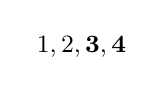
\begin{tikzpicture}
			\node at(0, 0){\small{$1,2,\mathbf{3},\mathbf{4}$}};
		\end{tikzpicture}
	\end{minipage}
	\begin{minipage}[t][2cm][c]{.15\textwidth}
		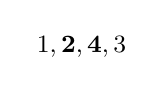
\begin{tikzpicture}
			\node at(0, 0){\small{$1,\mathbf{2},\mathbf{4},3$}};
		\end{tikzpicture}
	\end{minipage}
	\begin{minipage}[t][2cm][c]{.15\textwidth}
		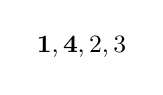
\begin{tikzpicture}
			\node at(0, 0){\small{$\mathbf{1},\mathbf{4},2,3$}};
		\end{tikzpicture}
	\end{minipage}
	\begin{minipage}[t][2cm][c]{.15\textwidth}
		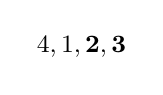
\begin{tikzpicture}
			\node at(0, 0){\small{$4,1,\mathbf{2},\mathbf{3}$}};
		\end{tikzpicture}
	\end{minipage}

	\begin{minipage}[t][2cm][c]{.15\textwidth}
		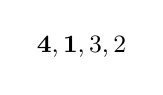
\begin{tikzpicture}
			\node at(0, 0){\small{$\mathbf{4},\mathbf{1},3,2$}};
		\end{tikzpicture}
	\end{minipage}
	\begin{minipage}[t][2cm][c]{.15\textwidth}
		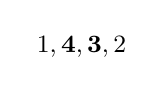
\begin{tikzpicture}
			\node at(0, 0){\small{$1,\mathbf{4},\mathbf{3},2$}};
		\end{tikzpicture}
	\end{minipage}
	\begin{minipage}[t][2cm][c]{.15\textwidth}
		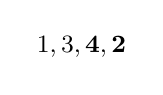
\begin{tikzpicture}
			\node at(0, 0){\small{$1,3,\mathbf{4},\mathbf{2}$}};
		\end{tikzpicture}
	\end{minipage}
	\begin{minipage}[t][2cm][c]{.15\textwidth}
		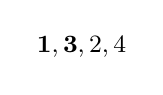
\begin{tikzpicture}
			\node at(0, 0){\small{$\mathbf{1},\mathbf{3},2,4$}};
		\end{tikzpicture}
	\end{minipage}

	\begin{minipage}[t][2cm][c]{.15\textwidth}
		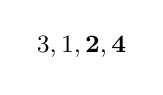
\begin{tikzpicture}
			\node at(0, 0){\small{$3,1,\mathbf{2},\mathbf{4}$}};
		\end{tikzpicture}
	\end{minipage}
	\begin{minipage}[t][2cm][c]{.15\textwidth}
		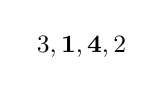
\begin{tikzpicture}
			\node at(0, 0){\small{$3,\mathbf{1},\mathbf{4},2$}};
		\end{tikzpicture}
	\end{minipage}
	\begin{minipage}[t][2cm][c]{.15\textwidth}
		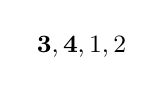
\begin{tikzpicture}
			\node at(0, 0){\small{$\mathbf{3},\mathbf{4},1,2$}};
		\end{tikzpicture}
	\end{minipage}
	\begin{minipage}[t][2cm][c]{.15\textwidth}
		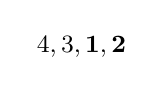
\begin{tikzpicture}
			\node at(0, 0){\small{$4,3,\mathbf{1},\mathbf{2}$}};
		\end{tikzpicture}
	\end{minipage}

	\begin{minipage}[t][2cm][c]{.15\textwidth}
		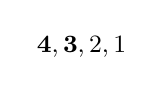
\begin{tikzpicture}
			\node at(0, 0){\small{$\mathbf{4},\mathbf{3},2,1$}};
		\end{tikzpicture}
	\end{minipage}
	\begin{minipage}[t][2cm][c]{.15\textwidth}
		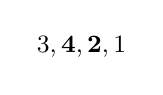
\begin{tikzpicture}
			\node at(0, 0){\small{$3,\mathbf{4},\mathbf{2},1$}};
		\end{tikzpicture}
	\end{minipage}
	\begin{minipage}[t][2cm][c]{.15\textwidth}
		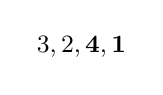
\begin{tikzpicture}
			\node at(0, 0){\small{$3,2,\mathbf{4},\mathbf{1}$}};
		\end{tikzpicture}
	\end{minipage}
	\begin{minipage}[t][2cm][c]{.15\textwidth}
		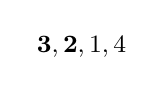
\begin{tikzpicture}
			\node at(0, 0){\small{$\mathbf{3},\mathbf{2},1,4$}};
		\end{tikzpicture}
	\end{minipage}

	\begin{minipage}[t][2cm][c]{.15\textwidth}
		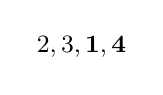
\begin{tikzpicture}
			\node at(0, 0){\small{$2,3,\mathbf{1},\mathbf{4}$}};
		\end{tikzpicture}
	\end{minipage}
	\begin{minipage}[t][2cm][c]{.15\textwidth}
		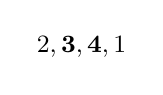
\begin{tikzpicture}
			\node at(0, 0){\small{$2,\mathbf{3},\mathbf{4},1$}};
		\end{tikzpicture}
	\end{minipage}
	\begin{minipage}[t][2cm][c]{.15\textwidth}
		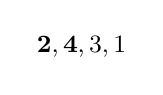
\begin{tikzpicture}
			\node at(0, 0){\small{$\mathbf{2},\mathbf{4},3,1$}};
		\end{tikzpicture}
	\end{minipage}
	\begin{minipage}[t][2cm][c]{.15\textwidth}
		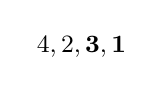
\begin{tikzpicture}
			\node at(0, 0){\small{$4,2,\mathbf{3},\mathbf{1}$}};
		\end{tikzpicture}
	\end{minipage}

	\begin{minipage}[t][2cm][c]{.15\textwidth}
		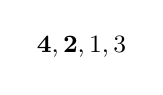
\begin{tikzpicture}
			\node at(0, 0){\small{$\mathbf{4},\mathbf{2},1,3$}};
		\end{tikzpicture}
	\end{minipage}
	\begin{minipage}[t][2cm][c]{.15\textwidth}
		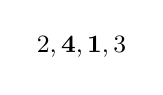
\begin{tikzpicture}
			\node at(0, 0){\small{$2,\mathbf{4},\mathbf{1},3$}};
		\end{tikzpicture}
	\end{minipage}
	\begin{minipage}[t][2cm][c]{.15\textwidth}
		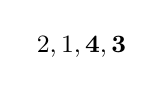
\begin{tikzpicture}
			\node at(0, 0){\small{$2,1,\mathbf{4},\mathbf{3}$}};
		\end{tikzpicture}
	\end{minipage}
	\begin{minipage}[t][2cm][c]{.15\textwidth}
		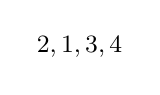
\begin{tikzpicture}
			\node at(0, 0){\small{$2,1,3,4$}};
		\end{tikzpicture}
	\end{minipage}
	
	\caption{$24$ permutations of order $4$ listed in Steinhaus-Johnson-Trotter Gray code order. Permutations are read 
	left to right, top to bottom.}
	\label{Fig:24Perms}
\end{figure} 
There are many known algorithms for listing permutations of order $n$. Throughout the course of this thesis,
a number of such algorithms were researched~\cite{A18,A19,A20,A24,A25,A26,A31,A34,A35,A36,A37}.
Each of these algorithms will be reviewed in Chapter 2. 
In Figure~\ref{Fig:24ladders}, one ladder per permutation is listed in lexicographic order; ladders are read left to right, top to bottom. 
We note that the lexicographic ordering of ladders is not a Gray code order. For example, transitioning from ladder 6 to ladder 7 in Figure~\ref{Fig:24ladders} 
requires four bars to be changed.\cleardoublepage


\begin{figure}[ht]
\centering
\begin{tikzpicture}
\draw(0.00,1.00) to (0.00,2.60);
\draw(0.50,1.00) to (0.50,2.60);
\draw(1.00,1.00) to (1.00,2.60);
\draw(1.50,1.00) to (1.50,2.60);
\node at(0.00,2.70){\tiny{1}};\node at(0.50,2.70){\tiny{2}};\node at(1.00,2.70){\tiny{3}};\node at(1.50,2.70){\tiny{4}};

\draw(4.00,1.00) to (4.00,2.60);
\draw(4.50,1.00) to (4.50,2.60);
\draw(5.00,1.00) to (5.00,2.60);
\draw(5.50,1.00) to (5.50,2.60);
\draw(5.00, 2.50) to (5.50, 2.50);
\node at(4.00,2.70){\tiny{1}};\node at(4.50,2.70){\tiny{2}};\node at(5.00,2.70){\tiny{4}};\node at(5.50,2.70){\tiny{3}};

\draw(8.00,1.00) to (8.00,2.60);
\draw(8.50,1.00) to (8.50,2.60);
\draw(9.00,1.00) to (9.00,2.60);
\draw(9.50,1.00) to (9.50,2.60);
\draw(8.50, 2.50) to (9.00, 2.50);
\node at(8.00,2.70){\tiny{1}};\node at(8.50,2.70){\tiny{3}};\node at(9.00,2.70){\tiny{2}};\node at(9.50,2.70){\tiny{4}};

\draw(12.00,1.00) to (12.00,2.60);
\draw(12.50,1.00) to (12.50,2.60);
\draw(13.00,1.00) to (13.00,2.60);
\draw(13.50,1.00) to (13.50,2.60);
\draw(13.00, 2.50) to (13.50, 2.50);
\draw(12.50, 2.20) to (13.00, 2.20);
\node at(12.00,2.70){\tiny{1}};\node at(12.50,2.70){\tiny{3}};\node at(13.00,2.70){\tiny{4}};\node at(13.50,2.70){\tiny{2}};

\draw(0.00,-1.50) to (0.00,0.10);
\draw(0.50,-1.50) to (0.50,0.10);
\draw(1.00,-1.50) to (1.00,0.10);
\draw(1.50,-1.50) to (1.50,0.10);
\draw(0.50, 0.00) to (1.00, 0.00);
\draw(1.00, -0.30) to (1.50, -0.30);
\node at(0.00,0.20){\tiny{1}};\node at(0.50,0.20){\tiny{4}};\node at(1.00,0.20){\tiny{2}};\node at(1.50,0.20){\tiny{3}};

\draw(4.00,-1.50) to (4.00,0.10);
\draw(4.50,-1.50) to (4.50,0.10);
\draw(5.00,-1.50) to (5.00,0.10);
\draw(5.50,-1.50) to (5.50,0.10);
\draw[line width=0.5mm, red](4.50, 0.00) to (5.00, 0.00);
\draw[line width=0.5mm, red](5.00, -0.30) to (5.50, -0.30);
\draw[line width=0.5mm, red](4.50, -0.60) to (5.00, -0.60);
\node at(4.00,0.20){\tiny{1}};\node at(4.50,0.20){\tiny{4}};\node at(5.00,0.20){\tiny{3}};\node at(5.50,0.20){\tiny{2}};

\draw(8.00,-1.50) to (8.00,0.10);
\draw(8.50,-1.50) to (8.50,0.10);
\draw(9.00,-1.50) to (9.00,0.10);
\draw(9.50,-1.50) to (9.50,0.10);
\draw[line width=.5mm, red](8.00, 0.00) to (8.50, 0.00);
\node at(8.00,0.20){\tiny{2}};\node at(8.50,0.20){\tiny{1}};\node at(9.00,0.20){\tiny{3}};\node at(9.50,0.20){\tiny{4}};

\draw(12.00,-1.50) to (12.00,0.10);
\draw(12.50,-1.50) to (12.50,0.10);
\draw(13.00,-1.50) to (13.00,0.10);
\draw(13.50,-1.50) to (13.50,0.10);
\draw(12.00, 0.00) to (12.50, 0.00);
\draw(13.00, 0.00) to (13.50, 0.00);
\node at(12.00,0.20){\tiny{2}};\node at(12.50,0.20){\tiny{1}};\node at(13.00,0.20){\tiny{4}};\node at(13.50,0.20){\tiny{3}};

\draw(0.00,-4.00) to (0.00,-2.40);
\draw(0.50,-4.00) to (0.50,-2.40);
\draw(1.00,-4.00) to (1.00,-2.40);
\draw(1.50,-4.00) to (1.50,-2.40);
\draw(0.50, -2.50) to (1.00, -2.50);
\draw(0.00, -2.80) to (0.50, -2.80);
\node at(0.00,-2.30){\tiny{2}};\node at(0.50,-2.30){\tiny{3}};\node at(1.00,-2.30){\tiny{1}};\node at(1.50,-2.30){\tiny{4}};

\draw(4.00,-4.00) to (4.00,-2.40);
\draw(4.50,-4.00) to (4.50,-2.40);
\draw(5.00,-4.00) to (5.00,-2.40);
\draw(5.50,-4.00) to (5.50,-2.40);
\draw(5.00, -2.50) to (5.50, -2.50);
\draw(4.50, -2.80) to (5.00, -2.80);
\draw(4.00, -3.10) to (4.50, -3.10);
\node at(4.00,-2.30){\tiny{2}};\node at(4.50,-2.30){\tiny{3}};\node at(5.00,-2.30){\tiny{4}};\node at(5.50,-2.30){\tiny{1}};

\draw(8.00,-4.00) to (8.00,-2.40);
\draw(8.50,-4.00) to (8.50,-2.40);
\draw(9.00,-4.00) to (9.00,-2.40);
\draw(9.50,-4.00) to (9.50,-2.40);
\draw(8.50, -2.50) to (9.00, -2.50);
\draw(8.00, -2.80) to (8.50, -2.80);
\draw(9.00, -2.80) to (9.50, -2.80);
\node at(8.00,-2.30){\tiny{2}};\node at(8.50,-2.30){\tiny{4}};\node at(9.00,-2.30){\tiny{1}};\node at(9.50,-2.30){\tiny{3}};

\draw(12.00,-4.00) to (12.00,-2.40);
\draw(12.50,-4.00) to (12.50,-2.40);
\draw(13.00,-4.00) to (13.00,-2.40);
\draw(13.50,-4.00) to (13.50,-2.40);
\draw(12.50, -2.50) to (13.00, -2.50);
\draw(13.00, -2.80) to (13.50, -2.80);
\draw(12.50, -3.10) to (13.00, -3.10);
\draw(12.00, -3.40) to (12.50, -3.40);
\node at(12.00,-2.30){\tiny{2}};\node at(12.50,-2.30){\tiny{4}};\node at(13.00,-2.30){\tiny{3}};\node at(13.50,-2.30){\tiny{1}};

\draw(0.00,-6.50) to (0.00,-4.90);
\draw(0.50,-6.50) to (0.50,-4.90);
\draw(1.00,-6.50) to (1.00,-4.90);
\draw(1.50,-6.50) to (1.50,-4.90);
\draw(0.00, -5.00) to (0.50, -5.00);
\draw(0.50, -5.30) to (1.00, -5.30);
\node at(0.00,-4.80){\tiny{3}};\node at(0.50,-4.80){\tiny{1}};\node at(1.00,-4.80){\tiny{2}};\node at(1.50,-4.80){\tiny{4}};

\draw(4.00,-6.50) to (4.00,-4.90);
\draw(4.50,-6.50) to (4.50,-4.90);
\draw(5.00,-6.50) to (5.00,-4.90);
\draw(5.50,-6.50) to (5.50,-4.90);
\draw(4.00, -5.00) to (4.50, -5.00);
\draw(5.00, -5.00) to (5.50, -5.00);
\draw(4.50, -5.30) to (5.00, -5.30);
\node at(4.00,-4.80){\tiny{3}};\node at(4.50,-4.80){\tiny{1}};\node at(5.00,-4.80){\tiny{4}};\node at(5.50,-4.80){\tiny{2}};

\draw(8.00,-6.50) to (8.00,-4.90);
\draw(8.50,-6.50) to (8.50,-4.90);
\draw(9.00,-6.50) to (9.00,-4.90);
\draw(9.50,-6.50) to (9.50,-4.90);
\draw(8.00, -5.00) to (8.50, -5.00);
\draw(8.50, -5.30) to (9.00, -5.30);
\draw(8.00, -5.60) to (8.50, -5.60);
\node at(8.00,-4.80){\tiny{3}};\node at(8.50,-4.80){\tiny{2}};\node at(9.00,-4.80){\tiny{1}};\node at(9.50,-4.80){\tiny{4}};

\draw(12.00,-6.50) to (12.00,-4.90);
\draw(12.50,-6.50) to (12.50,-4.90);
\draw(13.00,-6.50) to (13.00,-4.90);
\draw(13.50,-6.50) to (13.50,-4.90);
\draw(12.00, -5.00) to (12.50, -5.00);
\draw(13.00, -5.00) to (13.50, -5.00);
\draw(12.50, -5.30) to (13.00, -5.30);
\draw(12.00, -5.60) to (12.50, -5.60);
\node at(12.00,-4.80){\tiny{3}};\node at(12.50,-4.80){\tiny{2}};\node at(13.00,-4.80){\tiny{4}};\node at(13.50,-4.80){\tiny{1}};

\draw(0.00,-9.00) to (0.00,-7.40);
\draw(0.50,-9.00) to (0.50,-7.40);
\draw(1.00,-9.00) to (1.00,-7.40);
\draw(1.50,-9.00) to (1.50,-7.40);
\draw(0.50, -7.50) to (1.00, -7.50);
\draw(0.00, -7.80) to (0.50, -7.80);
\draw(1.00, -7.80) to (1.50, -7.80);
\draw(0.50, -8.10) to (1.00, -8.10);
\node at(0.00,-7.30){\tiny{3}};\node at(0.50,-7.30){\tiny{4}};\node at(1.00,-7.30){\tiny{1}};\node at(1.50,-7.30){\tiny{2}};

\draw(4.00,-9.00) to (4.00,-7.40);
\draw(4.50,-9.00) to (4.50,-7.40);
\draw(5.00,-9.00) to (5.00,-7.40);
\draw(5.50,-9.00) to (5.50,-7.40);
\draw(4.50, -7.50) to (5.00, -7.50);
\draw(4.00, -7.80) to (4.50, -7.80);
\draw(5.00, -7.80) to (5.50, -7.80);
\draw(4.50, -8.10) to (5.00, -8.10);
\draw(4.00, -8.40) to (4.50, -8.40);
\node at(4.00,-7.30){\tiny{3}};\node at(4.50,-7.30){\tiny{4}};\node at(5.00,-7.30){\tiny{2}};\node at(5.50,-7.30){\tiny{1}};

\draw(8.00,-9.00) to (8.00,-7.40);
\draw(8.50,-9.00) to (8.50,-7.40);
\draw(9.00,-9.00) to (9.00,-7.40);
\draw(9.50,-9.00) to (9.50,-7.40);
\draw(8.00, -7.50) to (8.50, -7.50);
\draw(8.50, -7.80) to (9.00, -7.80);
\draw(9.00, -8.10) to (9.50, -8.10);
\node at(8.00,-7.30){\tiny{4}};\node at(8.50,-7.30){\tiny{1}};\node at(9.00,-7.30){\tiny{2}};\node at(9.50,-7.30){\tiny{3}};

\draw(12.00,-9.00) to (12.00,-7.40);
\draw(12.50,-9.00) to (12.50,-7.40);
\draw(13.00,-9.00) to (13.00,-7.40);
\draw(13.50,-9.00) to (13.50,-7.40);
\draw(12.00, -7.50) to (12.50, -7.50);
\draw(12.50, -7.80) to (13.00, -7.80);
\draw(13.00, -8.10) to (13.50, -8.10);
\draw(12.50, -8.40) to (13.00, -8.40);
\node at(12.00,-7.30){\tiny{4}};\node at(12.50,-7.30){\tiny{1}};\node at(13.00,-7.30){\tiny{3}};\node at(13.50,-7.30){\tiny{2}};

\draw(0.00,-11.50) to (0.00,-9.90);
\draw(0.50,-11.50) to (0.50,-9.90);
\draw(1.00,-11.50) to (1.00,-9.90);
\draw(1.50,-11.50) to (1.50,-9.90);
\draw(0.00, -10.00) to (0.50, -10.00);
\draw(0.50, -10.30) to (1.00, -10.30);
\draw(0.00, -10.60) to (0.50, -10.60);
\draw(1.00, -10.60) to (1.50, -10.60);
\node at(0.00,-9.80){\tiny{4}};\node at(0.50,-9.80){\tiny{2}};\node at(1.00,-9.80){\tiny{1}};\node at(1.50,-9.80){\tiny{3}};

\draw(4.00,-11.50) to (4.00,-9.90);
\draw(4.50,-11.50) to (4.50,-9.90);
\draw(5.00,-11.50) to (5.00,-9.90);
\draw(5.50,-11.50) to (5.50,-9.90);
\draw(4.00, -10.00) to (4.50, -10.00);
\draw(4.50, -10.30) to (5.00, -10.30);
\draw(5.00, -10.60) to (5.50, -10.60);
\draw(4.50, -10.90) to (5.00, -10.90);
\draw(4.00, -11.20) to (4.50, -11.20);
\node at(4.00,-9.80){\tiny{4}};\node at(4.50,-9.80){\tiny{2}};\node at(5.00,-9.80){\tiny{3}};\node at(5.50,-9.80){\tiny{1}};

\draw(8.00,-11.50) to (8.00,-9.90);
\draw(8.50,-11.50) to (8.50,-9.90);
\draw(9.00,-11.50) to (9.00,-9.90);
\draw(9.50,-11.50) to (9.50,-9.90);
\draw(8.00, -10.00) to (8.50, -10.00);
\draw(8.50, -10.30) to (9.00, -10.30);
\draw(8.00, -10.60) to (8.50, -10.60);
\draw(9.00, -10.60) to (9.50, -10.60);
\draw(8.50, -10.90) to (9.00, -10.90);
\node at(8.00,-9.80){\tiny{4}};\node at(8.50,-9.80){\tiny{3}};\node at(9.00,-9.80){\tiny{1}};\node at(9.50,-9.80){\tiny{2}};

\draw(12.00,-11.50) to (12.00,-9.90);
\draw(12.50,-11.50) to (12.50,-9.90);
\draw(13.00,-11.50) to (13.00,-9.90);
\draw(13.50,-11.50) to (13.50,-9.90);
\draw(12.00, -10.00) to (12.50, -10.00);
\draw(12.50, -10.30) to (13.00, -10.30);
\draw(12.00, -10.60) to (12.50, -10.60);
\draw(13.00, -10.60) to (13.50, -10.60);
\draw(12.50, -10.90) to (13.00, -10.90);
\draw(12.00, -11.20) to (12.50, -11.20);
\node at(12.00,-9.80){\tiny{4}};\node at(12.50,-9.80){\tiny{3}};\node at(13.00,-9.80){\tiny{2}};\node at(13.50,-9.80){\tiny{1}};

\end{tikzpicture}
\caption{All 24 permutations listed in lexicographic order with a corresponding optimal ladder. Ladders are read left to right, top to bottom. Note how lex order is not a Gray code}
\label{Fig:24ladders}
\end{figure}


\section{Thesis Statement}
 We define \emph{The Canonical Ladder Listing Problem} as follows: 
Given $n$, provide a listing of $n!$ optimal ladders,
one corresponding to each permutation of order $n$, in Gray code order whereby successive ladders differ by a \emph{minimal amount of change}. 
First, we define \emph{minimal change} as either the addition  or removal of a bar. 
Second, we define \emph{minimal change} as moving a bar; moving a bar is the same as removing one bar and adding a new bar. 
We provide a canonical ladder representation of an optimal ladder from $OptL\{\pi\}$ in order to translate the ladder to a data structure. 
By doing so, we allow for a number of efficient solutions to solve The Canonical Ladder Listing Problem in the form of novel equations, 
algorithms, and Gray codes. 
	
	%%%Write a second part on ER if he decides you need it.

	

	

\section{Contributions}
In this thesis we provide the following contributions:
	\begin{enumerate}
    \item Definition of the canonical ladder.
    \item Definition of the data structure for the canonical ladder. 
    \item Function to calculate the location of a bar 
   in $O(1)$ time.
    \item $O(n^2)$ algorithm to create the canonical ladder corresponding to a given permutation.
    \item $O(1)$ amortized algorithm which lists $n!$ ladders where successive ladders differ by either a single  addition of a bar or a single removal of a bar.
    \item Gray code for listing ladders with $n$ lines and $k$ bars for some arbitrary $k$ value between $[0 \leq k \leq {n \choose 2}]$. 
    \item Gray code for listing $n!$ ladders ordered by the number of bars. Successive ladders differ by the relocation of a bar or by the 
    addition of a bar when transitioning from $k$ to $k+1$ bars.
\end{enumerate}
	

\section{Summary of Past Known Results}
To the best of my knowledge, the first paper written on ladder lotteries is titled Efficient Enumeration of 
Ladder Lotteries and its Application written by Yamanaka, Nakano, Matsui Uehara and Nakada. The paper 
was written in 2010~\cite{A1}. Since this paper, 
a number of problems related to ladder lotteries have been solved. In Table~\ref{Table:KnownProblems} 
the reader will find a table of solved problems related to ladder lotteries. In Chapter 2 a more comprehensive analysis of these 
solved problems will be provided.
\begin{table}[h]
	\centering
	\caption{Table of known solutions for problems related to ladder lotteries}
	\begin{tabular}{|p{4cm}||p{4cm}||p{4cm}|}
		\hline 
		\multicolumn{3}{|c|}{Table of Known Results Related to Ladder Lotteries}\\
		\hline 
		\hline 
		Name of Problem & Description & Source \\ 
		\hline 
		\small{Enumeration Problem} & \small{Generates $OptL\{\pi\}$} &~\cite{A1} 2010\\ 
		\hline
		\small{Ladder Lottery \newline Realization Problem} & \small{Determines time complexity for creating a ladder lottery given a multi-set of bars} &~\cite{A3} 2018\\ 
		\hline
		\small{The Reconfiguration \newline Problem} & \small{Determine the length of the path between two ladders in $OptL\{\pi\}$} &~\cite{A2} 2017\\ 
		\hline 
		\small{Enumeration Problem \newline given $n$, $k$} & \small{Generates all ladders with $n$ lines and $k$ bars; includes non-optimal ladders} &~\cite{A4} 2014\\ 
		\hline
		\small{The Coding Problem} & \small{Provides a binary string encoding for a ladder lottery} &~\cite{A5} 2012\\ 
		\hline 
		\small{Counting and \newline Random Generation \newline Problem} & \small{Provides a solution for counting ladder lotteries of a given type as well as randomly generating a ladder lottery} &~\cite{A6} 2017\\ 
		\hline
		
	\end{tabular}
	\label{Table:KnownProblems}
\end{table}

\section{Overview of Thesis}
This thesis is broken down into several sections. In Chapter 2, a literature
review of ladder lotteries will be provided along with background information pertinent to this thesis. 
In Chapter 3, a definition of the canonical ladder is provided 
along with the algorithm {\sc CreateCanonical}. 
In Chapter 4, an algorithm is provided which lists one optimal ladder corresponding to each permutation of order $n$ in Gray code order; 
a single bar is added or removed between successive ladders. 
In Chapter 5, an algorithm for listing all ladders with $n$ lines and $k$ bars in Gray code order is provided. 
Also in Chapter 5, we provide the algorithm for listing all $n!$ ladders ordered by the number of bars in Gray coder order. 